% Chapter Template

\chapter{Introduction} % Main chapter title

\label{Introduction}


\section{Biodiversity loss}

It is well documented that global biodiversity loss is accelerating, with anthropogenic factors often touted as the leading cause, either directly through deforestation and hunting, or indirectly through climate change and the introduction of invasive species, often rodents \citep{Chiarucci2011, Doherty2016, Newbold2015}. A meta-analysis by \cite{DeVos2015} gave a conservative estimate of current biodiversity loss as 1,000 times greater than the background 'natural' rate, with a magnitude of 10,000 times greater also plausible \citep{Ceballos2015}. This alarming rate of loss does not only affect the lost taxa themselves, it can also lead to extensive reduction in ecosystem multifunctionality, typically affecting poorer human communities \citep{Chiarucci2011, Allan2015, Fanin2018}.\\

\noindent Rainforests are no exception to this trend and in addition to the adverse effects of deforestation on biodiversity, its though that other forms of anthropogenic disturbance, such as vehicles, hunting, and light pollution, can double the biodiversity loss caused by deforestation alone \citep{Barlow2016}.

\section{Difficulties of measuring biodiversity and its loss}

Whilst it is universally agreed that biodiversity is being lost and almost universally agreed that anthropogenic factors are accelerating this process, measuring biodiversity and its loss can be inconsistent and even erroneous. Firstly, only about 15\% of all species have been described so we have no data concerning biodiversity loss for the vast majority of species on Earth. Secondly, of those that have been described, very little is known of their distribution, population size, ecology and life histories, with many species only known due to a single observation. Finally, of those species that have been described and documented to a greater extent, there are inconsistencies in survey methods and often a lack of baseline measures to compare to \citep{TheRoy2003}.  The ‘best’ survey method is often specific to a certain level of organisation and spatial scale of interest (e.g. satellite imagery and ground surveys for rainforest plant surveys). The rapid acceleration of biodiversity loss makes urgent the development of programmes to assess and monitor biodiversity suitable for large-scale ecological questions \citep{Chiarucci2011}.

\section{Passive audio monitoring and its advantages}

Passive audio monitoring (PAM) is becoming an increasingly popular method for large-scale biodiversity monitoring, primarily due to its relatively low cost \citep{Browning2017}. This involves deploying sound recorders in an environment and having them record for days or weeks at a time to either track a vocal species directly or to use a vocal species as a proxy for another species or the ecosystem as a whole. Previously, methods such as PAM have been greatly limited by lack of digitisation, high implementation costs and small data storage capacity \citep{Merchant2015}. However, advances over the last 10-15 years have improved these constraints dramatically and one audio sensor in particular that has been developed recently by a collaborative project between the University of Oxford and University of Southampton, AudioMoth, is making PAM not only viable option for monitoring biodiversity loss, but one of the best methods \citep{Hill2018}. More recently, multiple-microphone arrays are being used to spatially locate vocal species, improving population censoring \citep{Blumstein2011, Stevenson2015}.\\

\noindent In addition to the direct monitoring of biodiversity with PAM, PAM can also be used to track other acoustics which may be relevant to conservationists, such as gunshots which are generally associated with illegal hunting, particularly in protected areas. \cite{Astaras2017} used PAM in a national park in Cameroon to successfully monitor the rates of hunting in the area. They found most (68.6\%) hunting occurred at night when ranger patrols were minimal and that there was more illegal activity during the week, probably due to the typical Saturday market days, implying this hunting was for the illegal mate trade rather than for sustinance or sport. However, \cite{Astaras2017} noted that the cost of equipment for PAM was quite high, and that this may limit its implementation in other national parks. The recent development of much cheaper audio sensors by \cite{Hill2018} may aid the spread of these techniques in conservation.

\section{Analysis of audio data}

Sound is the propagation of waves of pressure through a medium. When a gun is fired, the vibrations produced alternately compress and rarefy the medium, leading to waves of high and low pressure that propagate in all directions \citep{Bradbury2011}. Over time and distance, these waves attenuate, that is their amplitude reduces as energy dissipates into the environment \citep{Russ2013}.


To capture this data electronically, sound waves are transduced into an electrical signal with amplitude proportional to the amplitude of the sound wave through the vibration of the diaphragm of a microphone. Previously, the transduced electrical signal was then recorded directly onto an analogue tape but digitisation has become far more frequently used due to it allowing much longer recording times, with the data then being in a more appropriate format for computer analysis. To record digitally, the analog signal is sampled at a certain rate (typically measured in thousands of samples per second, kHz) and bit-depth (number of possible amplitude levels, typically 16-bit), with both parameters being important for determining frequency and amplitude resolution respectively. The signal information is then electronically recorded in the time-amplitude domain and can be processed mathematically using a fast Fourier transform (FFT) to convert the amplitude data into frequency data. For a given time window in the recording, the FFT calculates the frequency components of the signal and their relative amplitudes, producing a frequency spectrum. For a visual representation of the whole recording, an FFT is calculated with an overlapping short sliding window across the length of the recording, producing a spectrogram \citep{TheRoy2003} This entire process is outlined in Figure ~\ref{fig:audio_analysis}.\\

\begin{figure}
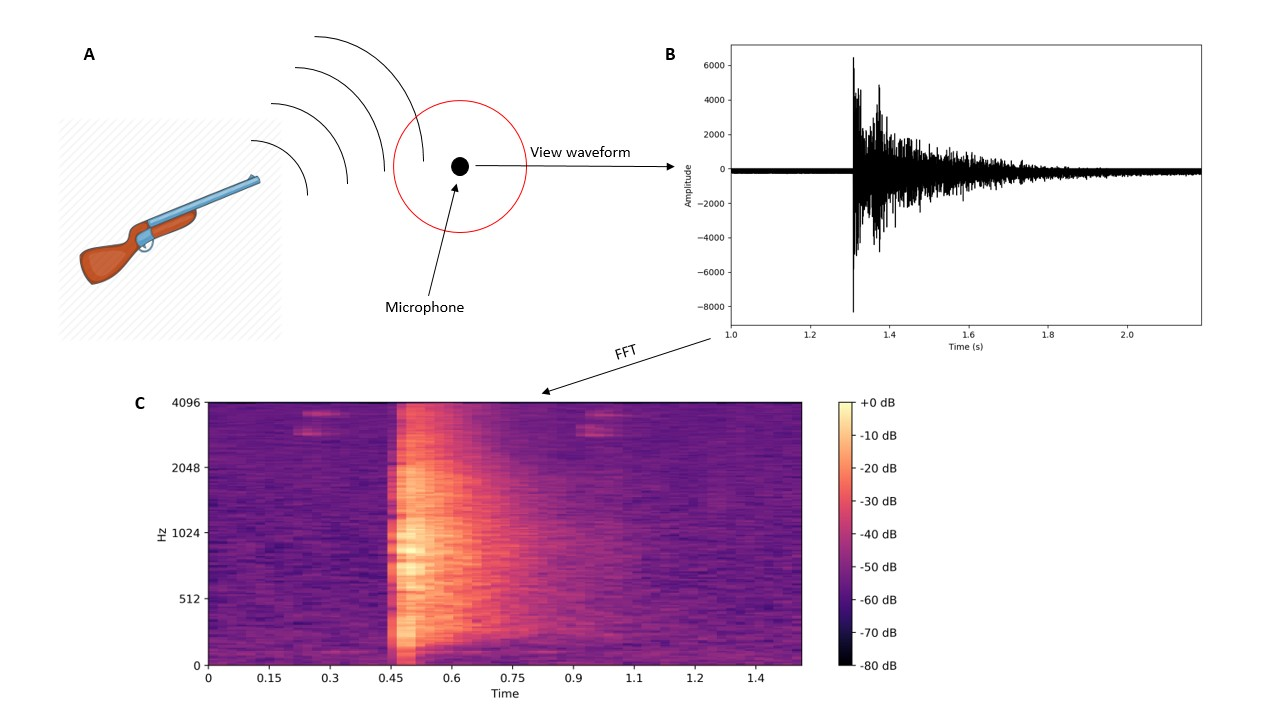
\includegraphics[width=1.2\textwidth,center]{Figures/audio_analysis}\caption[Analysis of acoustic data]{Recording and analysis of an acoustic signal. The emitted sound is transduced into an electrical signal by a microphone (\textbf{A}). In digital recording, the sound can be reconstructed in the time-amplitude domain (\textbf{B}) using the specified sampling rate (kHz). A frequency spectrum can then be produced using a fast Fourier transform (FFT), which calculates the signal’s frequency components and their relative amplitudes. Calculating FFT within a sliding window across the recording produces a spectrogram, with time on the x-axis, frequency on the y-axis, and with amplitude (energy) shown as colour intensity (\textbf{C})}\label{fig:audio_analysis}
\end{figure}


\noindent It is common in audio classification to plot a variant of the traditional spectrogram, the mel-frequency spectrogram. This involves calculating the mel-frequency cepstrum (MFC) which is a representation of the sound's power spectrum after the frequency has passed through a mathematical function. Mel-frequency cepstral coefficients (MFCCs) are the constiuent coefficients of an MFC \citep{Xu2004}. They are calculated from a cepstral representation of the sound, with frequency bands equally spaced on the mel scale \citep{Stevens1937}. \\


\noindent Spectrograms are fundamental to the analysis of acoustic data as they allow very specific sounds (e.g. spider monkey call, gunshot) to be visually identified and labelled, either manually or automatically.

\section{Machine learning}

Once audio data are collected, ecological information can be extracted manually or automatically. Manual extraction involves an expert either auditorily or visually inspecting the data and classifying the desired sounds, naturally incurring some bias based on their skill \citep{Heinicke2015}. This may be a viable option with a skilled ecologist and a small dataset but the latter is becoming increasingly rare with technological advances, therefore the need for automated techniques is growing. Fortunately, automated techniques are improving rapidly in accuracy and efficiency, largely due to the use of machine learning \citep{Digby2013}. Most automated tools utilise supervised machine learning and related methods, including artificial neural networks \citep{Walters2012}, random forest \citep{ZamoraGutierrez2016}, Hidden Markov Models \citep{Zilli2014}, and support vector machines \citep{Heinicke2015}. These methods commonly use libraries of species calls or other sounds to facilitate detection when presented with new recordings. Currently, the accuracy of these systems is rarely good enough to enable full automation and manual validation is often required \citep{Kalan2016}. However, new methods such as unsupervised feature extraction \citep{Stowell2014} and deep convolutional neural networks \citep{Goeau2016} can learn to classify directly from spectrogram data, often making them more robust and resistant to noise. At present, the main limitation for deep convolutional neural networks is large, clean datasets to train on.

\section{Costa Rica and conservation}

Costa Rica is no exception to the aforementioned trend of biodiversity loss, with the Osa Peninsula being an area of focus for recent studies as it contains a mixture of protected, partially-protected and unprotected land \citep{Lawson2019}. Whilst protected areas have benefited some species, others such as the Geoffroy’s spider monkey, \textit{Ateles Geoffroyi}, are struggling due to their diet and need for mature trees which is increasingly limiting their range and may be isolating populations, limiting their survival and genetic variability \citep{Chapman1989}. \textit{A. geoffroyi} is classified as endangered by the IUCN due to a 50\% reduction in numbers of the last 45 years \citep{Cuaron2008}. This reduction may be having a negative impact on other species as \textit{A. geoffroyi} is known to disperse the seeds of up to 150 different tree species \citep{VanRoosmalen1985}. As well as this habitat fragmentation, \textit{A. geoffroyi} is being subjected to hunting in both protected and non-protected areas. \cite{Aquino2013} found hunted populations of \textit{A. geoffroyi} in Peru were 70-80\% less dense than non-hunted populations. However, the monitoring and prevention of hunting in protected areas is often difficult in large reserves with limited resources available to rangers and conservationists, but a recent study by \cite{Hill2018} demonstrated gunshots can be detected with acoustic sensors up to 1 km from the source, opening a potentially cheaper and more effective mitigation strategy.

\section{Aims}

\begin{enumerate}
  \item To use data provided by \cite{Hill2018} to train a deep convolutional neural network that can detect gunshots in acoustic data
  \item To investigate the effectiveness of using machine learning in cases such as this
  \item To identify the presence of any spatio-temporal patterns of hunting in the Osa Peninsula
\end{enumerate}
